\section{RESULTS AND DISCUSSION} \label{sec:results}

In this section, the obtained control strategies are applied to a finite-difference method (FDM) representation of the system to evaluate its dynamic response. The system is discretized in space using a uniform grid with 100 equidistributed points, resulting in a system of ordinary differential equations (ODEs) with respect to time. This spatial discretization is introduced solely at the evaluation stage to numerically approximate the system's behavior under the influence of the optimal control input and is not involved in the design of the control law. The control law is derived directly in the infinite-dimensional space, fully capturing the continuous nature of the original system.

To solve the resulting ODEs, an adaptive Runge-Kutta method of order 5(4), commonly referred to as RK45, is employed. This method dynamically adjusts time steps to balance accuracy and computational efficiency, ensuring a reliable numerical solution while evaluating the system at specific points as required \autocite{RK45_1, RK45_2}. The implementation of this method is facilitated using the \texttt{solve\_ivp} function from Python's \texttt{SciPy} library \autocite{2020SciPy}, which provides a robust framework for handling time integration of ODEs.

Employing the outlined approach to evaluate the dynamic response of the systems under consideration, a comparative analysis is conducted between two identical systems with full-state access, differing only in the number of eigenmodes employed to compute the optimal full-state feedback gains. Subsequently, the performance of the proposed observer-based controller is assessed, with particular attention given to the dynamics of state reconstruction errors. Finally, a sensitivity analysis is performed to examine the impact of key parameters on the model behavior and the effectiveness of the control strategy. Across all simulations presented, $\mathfrak{Q} = 0.05 \cdot \mathfrak{I}$ and $\mathfrak{R} = 50$ are used as the deviation penalty and control effort weight operators, respectively, where $\mathfrak{I}$ denotes the identity operator matching the size of $\mathfrak{A}$.

% The obtained controller strategies in the previous section are applied to a finite-difference method (FDM) representation of the system model to evaluate the system dynamics. The system model is discretized in space and time, and the resulting system of ordinary differential equations is solved using the \texttt{`solve\_ivp'} function in Python's \texttt{`SciPy'} library \autocite{2020SciPy}, which employs the adaptive Runge-Kutta method of order 5(4), \texttt{`RK45'}. Each state of the system is discretized in space using 100 grid points. The \texttt{`RK45'} method automatically adjusts time steps to balance accuracy and computational efficiency, with the solution being evaluated at specific points as required \autocite{RK45_1,RK45_2}. First, the unstable dynamics of the open-loop system is explored. Then two full-state feedback systems are compared with respect to number of eigenmodes used to obtain the optimal feedback gain. Finally, the performance of the proposed observer-based controller is evaluated and the state reconstruction error dynamics are analyzed. 
% In all simulations presented, $\mathfrak{Q} = 0.05 \cdot \mathfrak{I}$ and $\mathfrak{R} = 50$ are used as the deviation penalty and control effort weight operators, respectively. Here, $\mathfrak{I}$ denotes the identity operator matching the size of $\mathfrak{A}$.

% \subsection{FDM representation of the open-loop system}

% Zero-input response of the system is explored using the mentioned FDM setup to show the unstable dynamics of the model. The state profile versus time and space $x_1(\zeta,t)$, is illustrated in Figure~\ref{fig:3D_x1_openloop}. The goal is to stabilize the system using an optimal control strategy. The system is unstable as the result of the generation term in the model.

% \begin{figure}[!htbp]
%     \centering
%     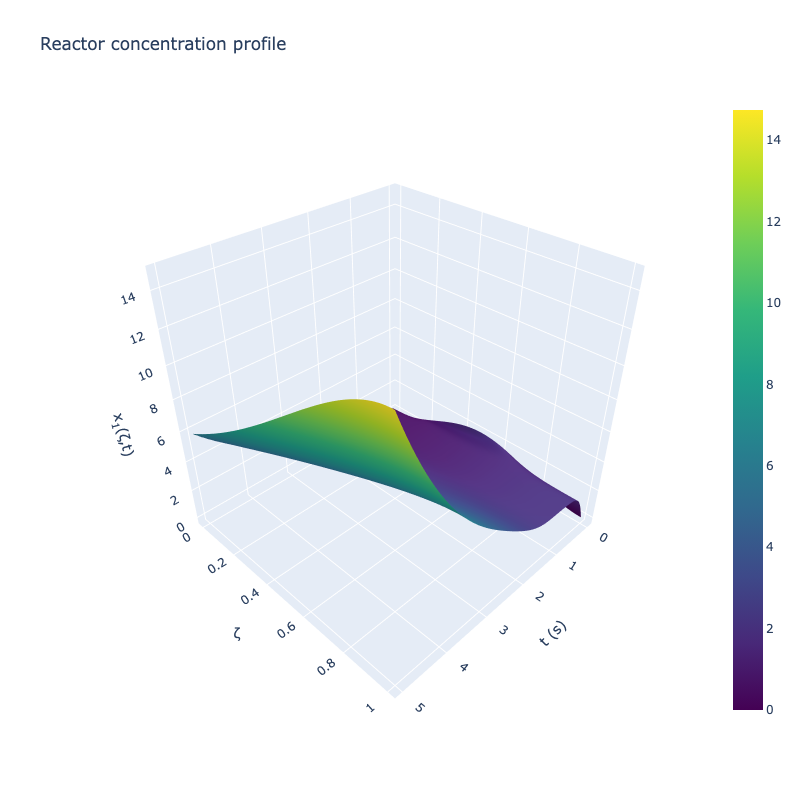
\includegraphics[width=0.8\textwidth,trim=0 0 100 0,clip]{Figures/3D_x1_openloop.png}
%     \caption{Zero-input response of the unstable open-loop system as described by Equations~(\ref{eq:PDE_original_model})~and~(\ref{eq:BC}).}
%     \label{fig:3D_x1_openloop}
% \end{figure}

\subsection{Full-state feedback regulator FDM representation}


Initially, the input response of the system provided by the full-state feedback is explored using the mentioned FDM setup. Two configurations are compared where the optimal feedback gain is obtained using different number of eigenmodes: one with $N=3$ and another with $N=7$, according to Figure~\ref{fig:k_modes}. The state profile versus time and space is illustrated for both cases in Figure~\ref{fig:full_state_feedback}. 

\begin{figure}[!htbp]
    \centering
    \begin{subfigure}[b]{0.45\textwidth}
        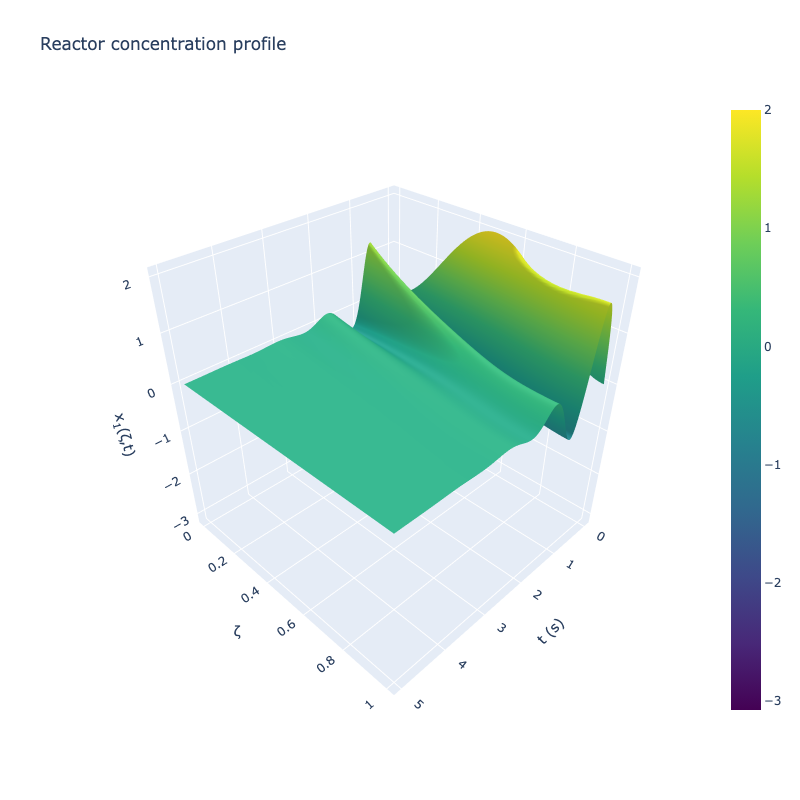
\includegraphics[width=\textwidth,trim=0 0 100 0,clip]{Figures/3D_x1_k3.png}
        \caption{$N=3$}
        \label{fig:3D_x1_k3}
    \end{subfigure}
    \hfill
    \begin{subfigure}[b]{0.45\textwidth}
        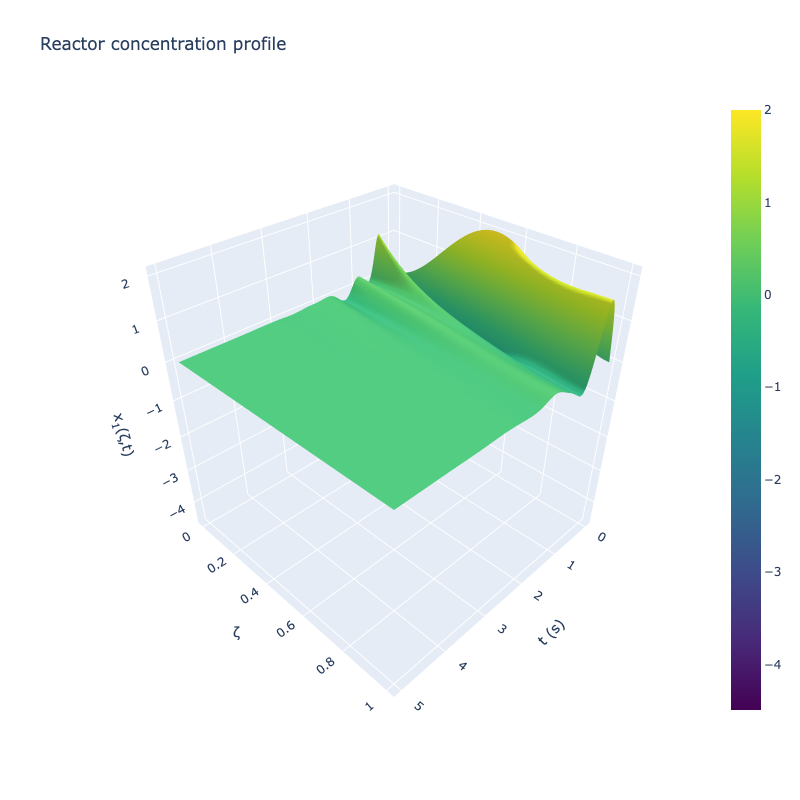
\includegraphics[width=\textwidth,trim=0 0 100 0,clip]{Figures/3D_x1_k7.png}
        \caption{$N=7$}
        \label{fig:3D_x1_k7}
    \end{subfigure}
    \caption{Input response of the system under full-state feedback control given by Equation~(\ref{eq:fullstate_ss}), utilizing the feedback gain obtained in Figure~\ref{fig:k_modes}.}
    \label{fig:full_state_feedback}
\end{figure}

In order to offer a clearer representation of the state trajectory in time, spatial cross-sectional plots are provided in Figure~\ref{fig:2D_xt_k7} for the $N=7$ case at different lengths of the domain. The delay-imposing state, i.e. the concentration along the recycle stream $x_2(\zeta,t)$, is provided only in Figure~\ref{fig:2D_xt_k7} for the sake of conciseness.

\begin{figure}[!htbp]
    \centering
    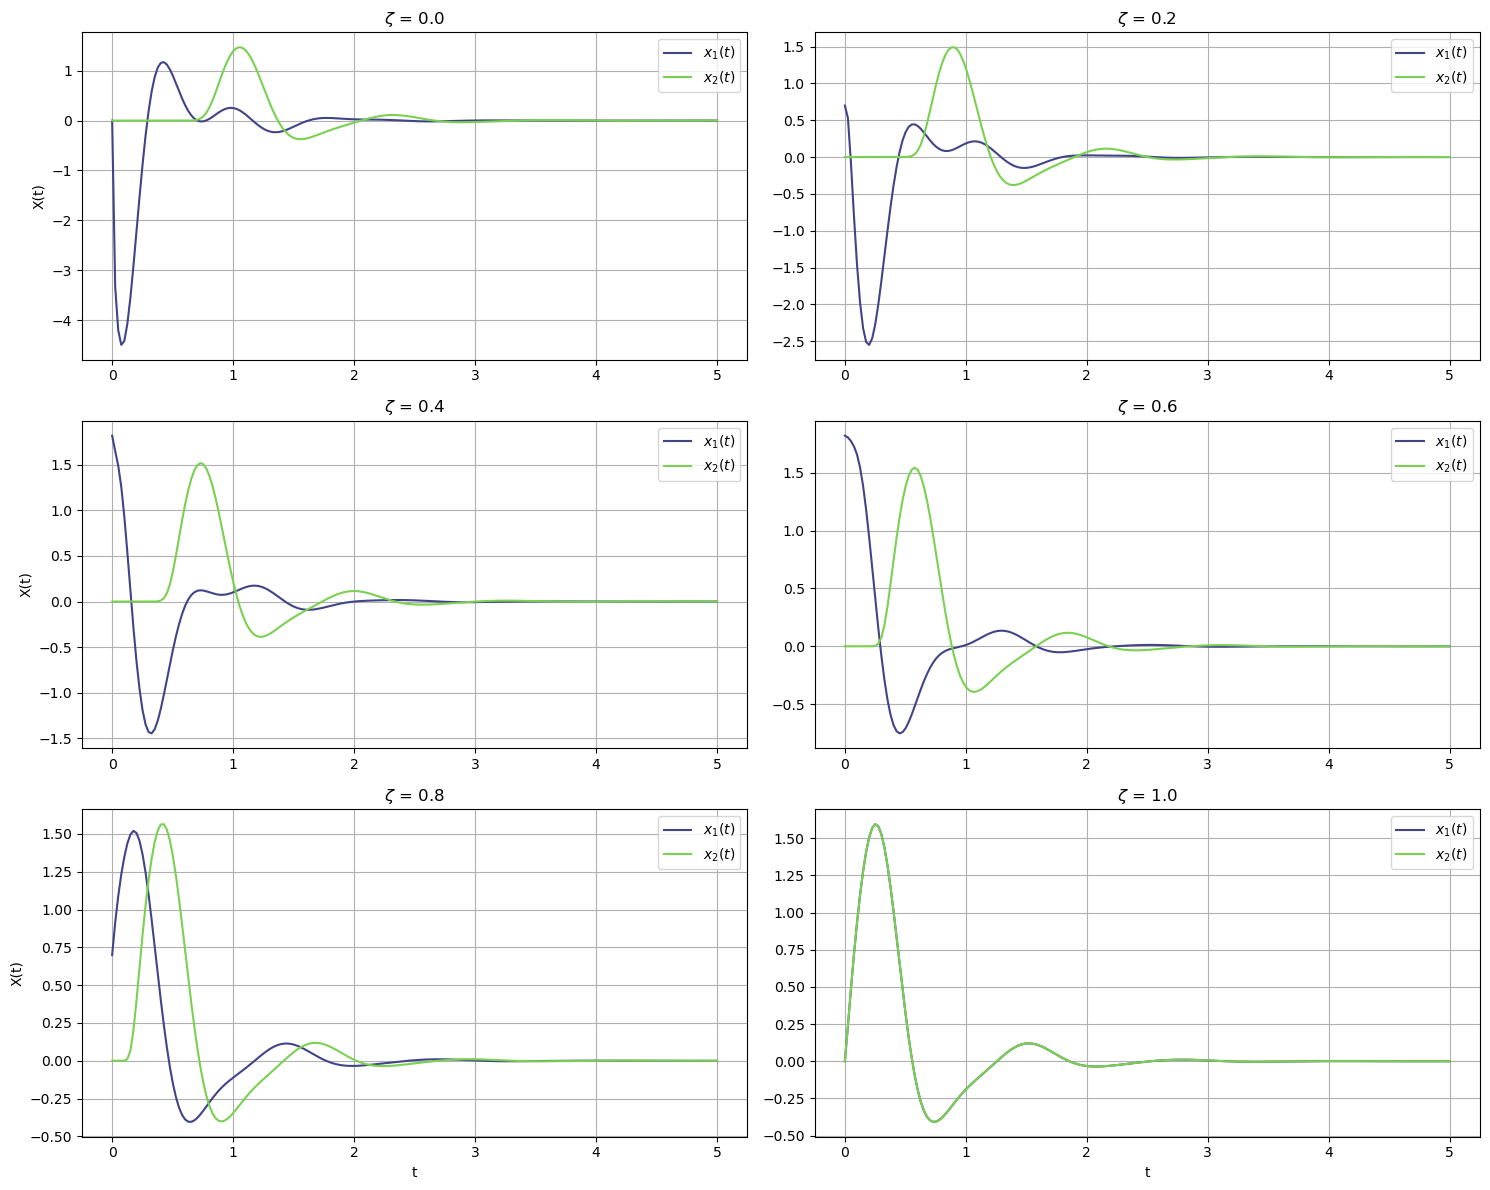
\includegraphics[width=0.8\textwidth]{Figures/2D_xt_k7.png}
    \caption{2D cross-section plots of the full-state feedback input response at various $\zeta$ positions, utilizing the feedback gain obtained in Figure~\ref{fig:k_7}.}
    \label{fig:2D_xt_k7}
\end{figure}

Both optimal feedback gains are able to successfully stabilize the system within finite time horizon. However, the case where more eigenmodes are considered in the controller design shows better performance, as the higher dimensional controller is able to stabilize the system quicker with lower cost function values in general.

\subsection{Observer-based regulator FDM representation} \label{sec:observer}

Omitting the need to have full access to system states, the observer-based regulator is evaluated using the same FDM representation. The states reconstruction is done by applying the observer gain obtained in Figure~\ref{fig:L_modes} to the system output. The estimated states are now used with the previously obtained optimal feedback gain with $N=7$ eigenmodes to calculate the input. Similar to the previous case, the state profile $x_1(\zeta,t)$ is illustrated in Figure~\ref{fig:3D_x1_L_k7}, as well as cross-sectional plots for both states in Figure~\ref{fig:2D_xt_L_k7} for better visualization of state trajectories in time.

\begin{figure}[!htbp]
    \centering
    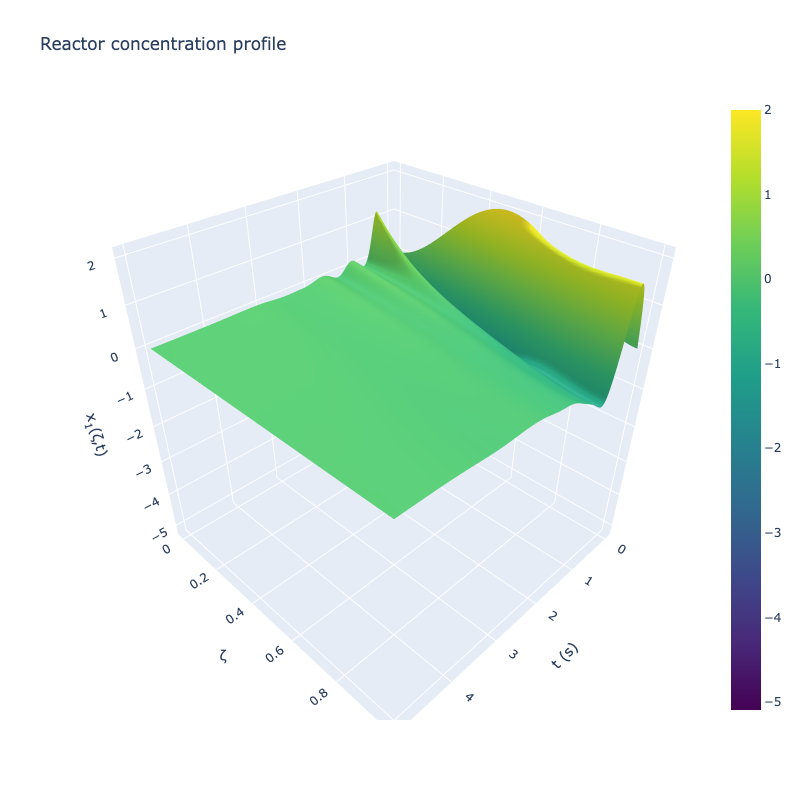
\includegraphics[width=0.8\textwidth,trim=0 0 100 0,clip]{Figures/3D_x1_L_k7.png}
    \caption{Input response of the system under observer-based output feedback control given by Equation~(\ref{eq:observer_ss}), utilizing the observer gain obtained in Figure~\ref{fig:L_modes} and the feedback gain obtained in Figure~\ref{fig:k_7}.}
    \label{fig:3D_x1_L_k7}
\end{figure}

\begin{figure}[!htbp]
    \centering
    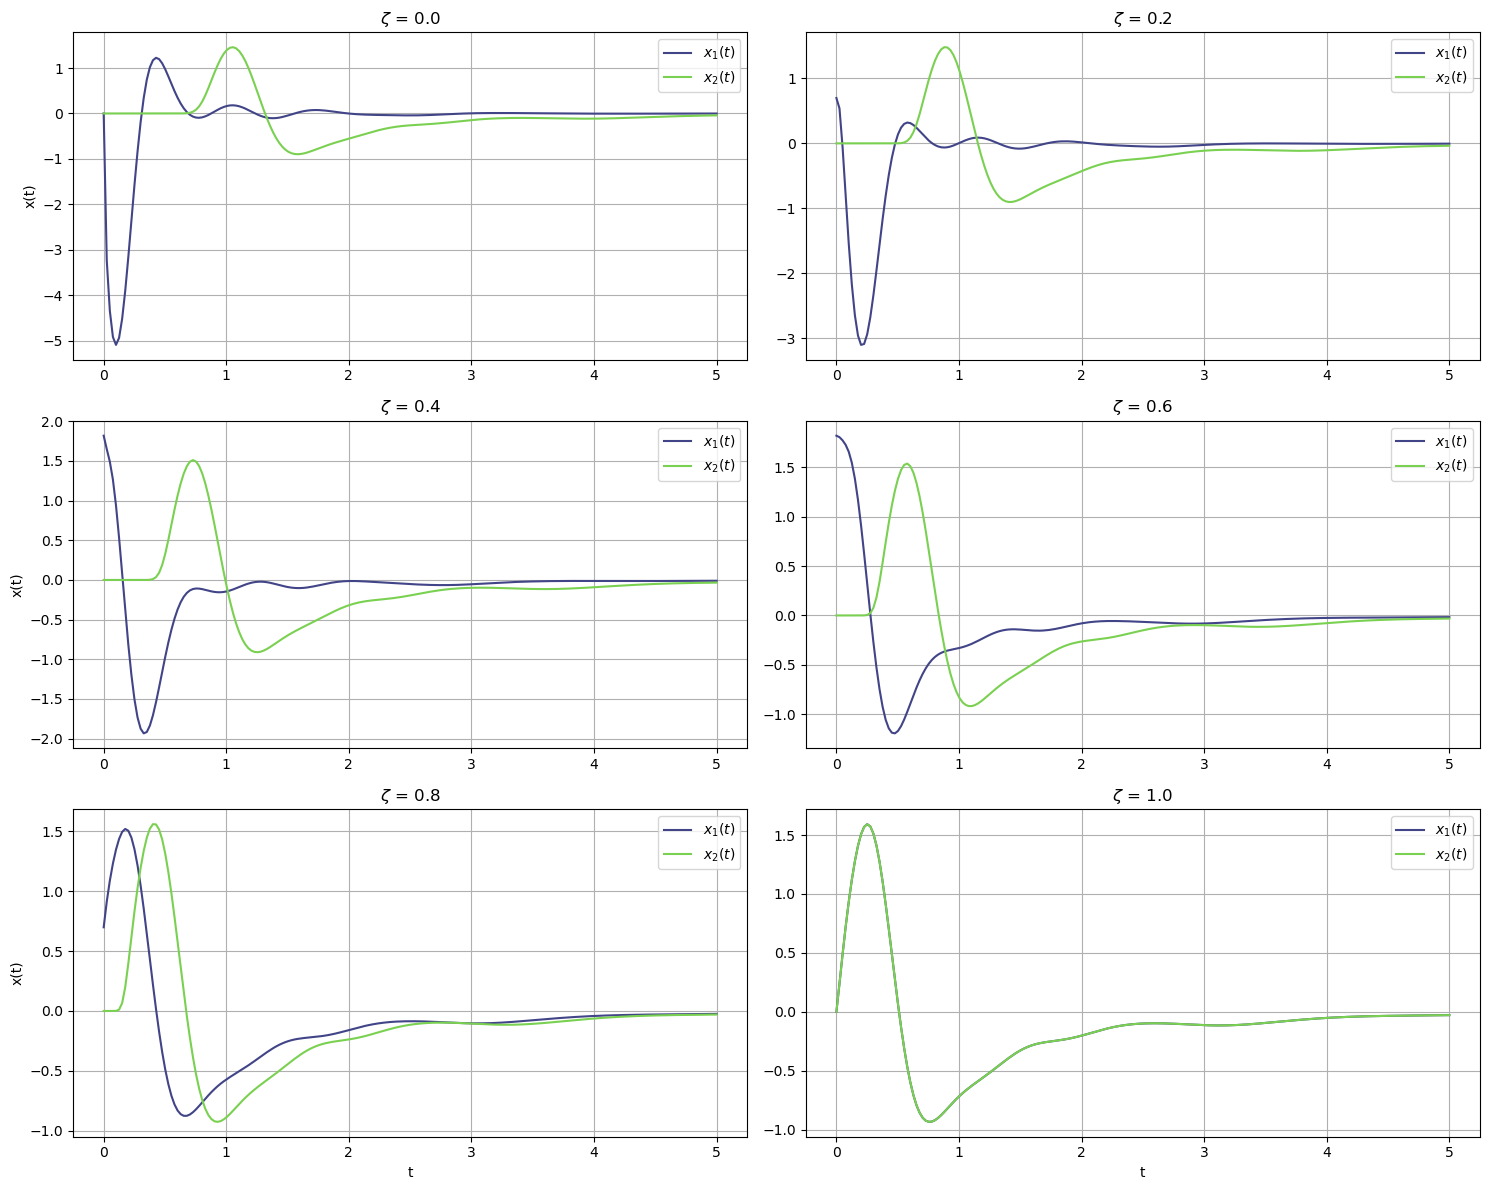
\includegraphics[width=0.8\textwidth]{Figures/2D_xt_L_k7.png}
    \caption{2D cross-section plots of the input response at various $\zeta$ positions, utilizing the observer gain obtained in Figure~\ref{fig:L_modes} and the feedback gain obtained in Figure~\ref{fig:k_7}.}
    \label{fig:2D_xt_L_k7}
\end{figure}

In the next step, the state estimation error dynamics of the observer are plotted in Figures~\ref{fig:3D_e1_L_k7}~and~\ref{fig:2D_et_L_k7} to demonstrate the performance of the observer. The error dynamics are calculated as the squared difference between the true state and the estimated state at each grid point and time instance.

\begin{figure}[!htbp]
    \centering
    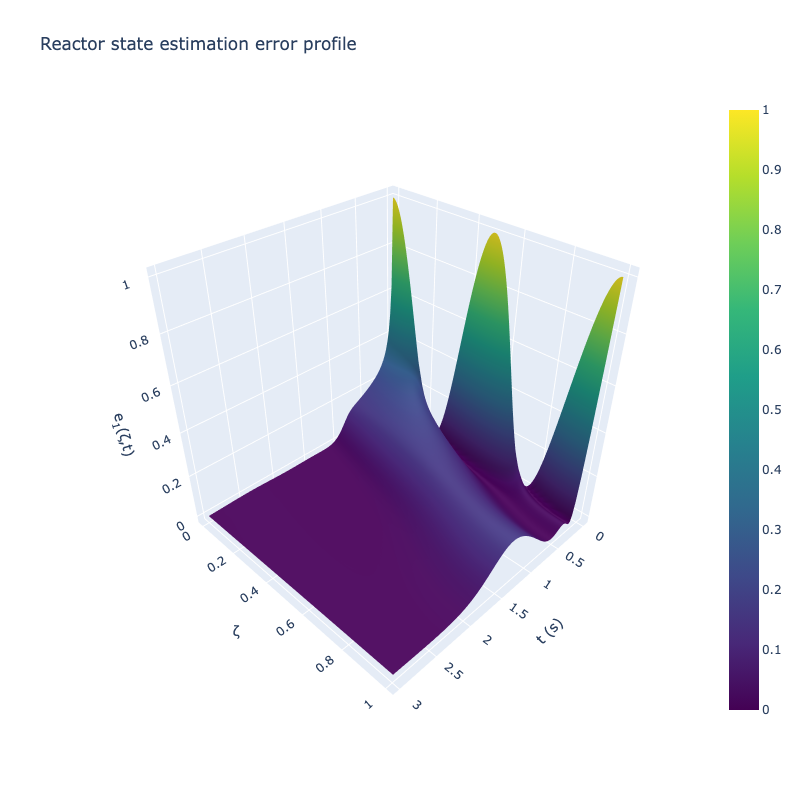
\includegraphics[width=0.8\textwidth,trim=0 0 100 0,clip]{Figures/3D_e1_L_k7.png}
    \caption{Error dynamics of the observer-based regulator utilizing the observer gain obtained in Figure~\ref{fig:L_modes} and the feedback gain obtained in Figure~\ref{fig:k_7}.}
    \label{fig:3D_e1_L_k7}
\end{figure}

\begin{figure}[!htbp]
    \centering
    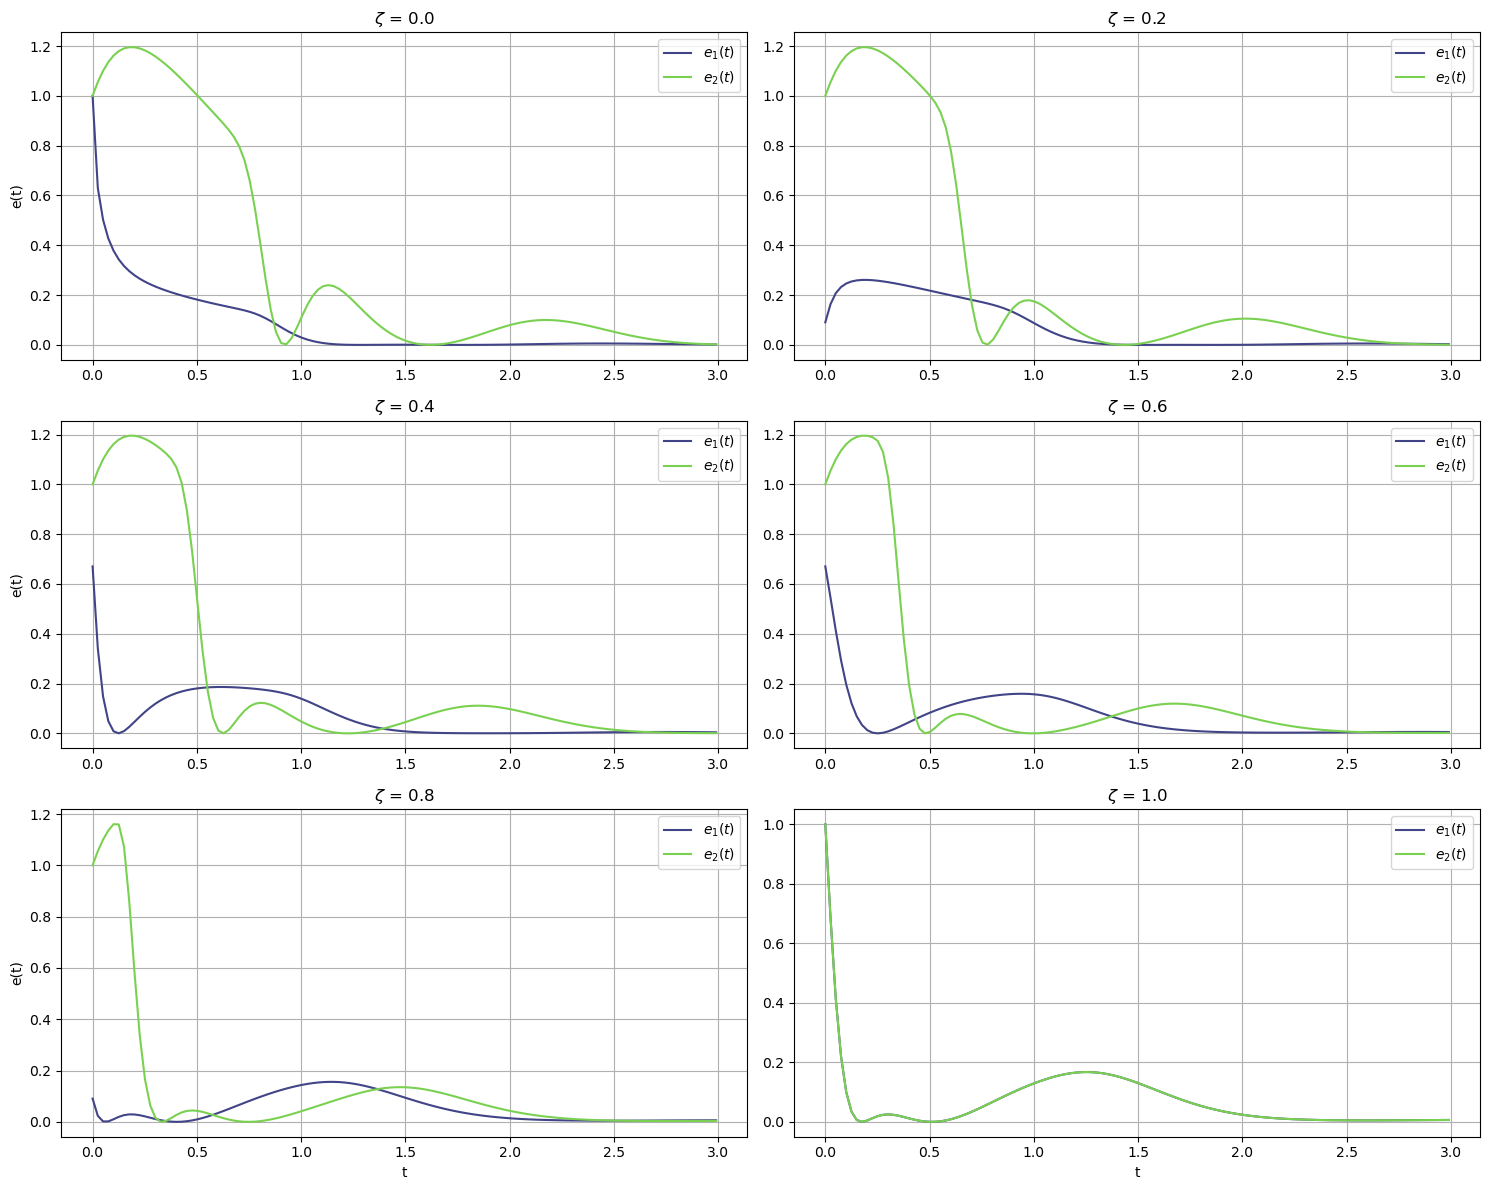
\includegraphics[width=0.8\textwidth]{Figures/2D_et_L_k7.png}
    \caption{2D cross-section plots of the error dynamics of the observer-based regulator at various $\zeta$ positions, utilizing the observer gain obtained in Figure~\ref{fig:L_modes} and the feedback gain obtained in Figure~\ref{fig:k_7}.}
    \label{fig:2D_et_L_k7}
\end{figure}

While the performance of the observer-based controller is slightly more sluggish compared to that of the full-state feedback regulator, it successfully stabilizes the system within a finite time horizon using only output measurements instead of full state information. In the absence of uncertainty in the system model, the observer gain can theoretically be designed so that the state estimation error converges to zero very fast compared to full-state feedback regulator dynamics. In practice, however, the observer gain is constrained by factors such as noise in the system output and plant-model mismatches. Despite these challenges, the proposed observer design mechanism achieves system stabilization with reasonable performance.

\subsection{Parameter sensitivity analysis}

Followed by showcasing the ability of the proposed controller to stabilize an unstable system using merely output measurements, a brief parameter sensitivity analysis of the model dynamics and controller performance is conducted at the end of this section. The effects of varying the recycle ratio $R$ and mass transfer Peclet number (i.e. the ratio of convection to diffusion, $Pe = v/D$) were explored during initial simulations. In addition, as it is central to this work, the effect of varying time delay $\tau$ on the response of the system under the original controller design is investigated in more detail.

Regarding the effect of recycle ratio on system dynamics and controller performance, it was observed that as the recycle ratio approaches unity, the open-loop system exhibits behavior similar to that of a well-mixed reactor, with concentration profiles flattening. This also influences the controller performance as it becomes more challenging to affect the system dynamics with the control input as the controller's action becomes diluted at the reactor inlet due to mixing with the recycle stream. For changes in mass Peclet number and its effect on the system dynamics, it was observed that a decrease in the Peclet number causes the eigenvalues of the system generator to shift closer to the real axis of the complex plane. This implies that greater diffusion relative to convection dampens the oscillatory behavior of the system that is originally imposed as the result of the delayed recycle stream.

Finally, the effect of varying time delay $\tau$ on the system dynamics is also investigated, as it is a key parameter in the model and controller design within this work. Input responses of several systems with different time delays are compared in Figure~\ref{fig:tau_sensitivity}, where the input for all cases is calculated assuming $\tau = 80$ s, which results in the same output feedback gain as the one obtained in \textbf{Section~\ref{sec:observer}}.

\begin{figure}[!htbp]
    \centering
    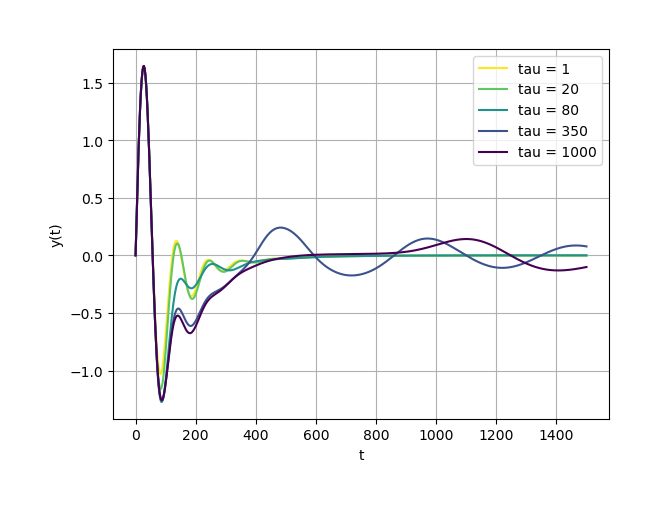
\includegraphics[width=0.8\textwidth]{Figures/y_vs_t.png}
    \caption{Measured output of the systems with different time delays $\tau$, under observer-based output feedback control utilizing the observer gain obtained in Figure~\ref{fig:L_modes} and the feedback gain obtained in Figure~\ref{fig:k_7}, where $\tau = 80$ s.}
    \label{fig:tau_sensitivity}
\end{figure}

It can be seen that as long as the actual time delay of a system is less than the assumed delay used in the controller design, the controller is still able to stabilize the system within a finite time horizon, although transient deviations from the desired behavior are observed. However, as the actual delay increases, the response of the system starts to deviate significantly from the desired behavior, especially after a certain threshold close to the actual recycle delay of the system. This shows the importance of including the time delay in the controller design to ensure the stability of the system within an optimal framework.

Although further parameter sensitivity analysis is possible as it naturally raises readers' curiosity, expanding the analysis to include more detailed investigations would risk exceeding the scope of this work, which is to offer a novel modeling and control framework for a certain class of distributed parameter systems in chemical engineering. Nonetheless, the proposed modeling and control strategy is able to effectively stabilize the system over a broad range of parameter sets, including but not limited to variations in the imposed time delay, Peclet number, and recycle ratio, ensuring the practicality of the proposed framework across different system configurations.